\documentclass[11pt,a4paper,useAMS,iop]{emulateapj}

\usepackage{tikz}
\usetikzlibrary{arrows,shapes,backgrounds}

\usepackage{xcolor}
\usepackage{threeparttable}
\usepackage{multirow}
\usepackage[colorlinks=true,linkcolor=blue,anchorcolor=blue,citecolor=blue,urlcolor=blue,draft=false]{hyperref}
\bibliographystyle{apj}
\usepackage{amsmath}
\usepackage{graphicx}
\usepackage{morefloats}
\usepackage{natbib}
\usepackage[percent]{overpic}
\usepackage{enumerate}
\usepackage{sidecap}
\usepackage{array}

\newcommand{\vdag}{(v)^\dagger}
\newcommand{\myemail}{gogrean@stanford.edu}

\slugcomment{Submitted to ApJ. Draft version dated \today.}

\shorttitle{The Large-Scale Filament Crossing MACS J0717.5+3745}
\shortauthors{Ogrean et al.}

\newcommand{\chandra}{\emph{Chandra}}
\newcommand{\rosat}{\emph{ROSAT}}
\newcommand{\vla}{\emph{VLA}}
\newcommand{\xmm}{\emph{XMM-Newton}}
\newcommand{\suzaku}{\emph{Suzaku}}
\newcommand{\gmrt}{\emph{GMRT}}
\newcommand{\wsrt}{\emph{WSRT}}

\begin{document}

\title{Frontier Fields Clusters: Properties of the X-ray-Bright Gas \\in the Large-Scale Filament Crossing MACS J0717.5+3745}

\author{
G.~A.~Ogrean\altaffilmark{1, $\dagger$}, C.~Jones\altaffilmark{2}, T.~Whalen\altaffilmark{3}, R.~J.~van Weeren\altaffilmark{2, $\ddagger$}, N.~Werner\altaffilmark{1}, W.~Forman\altaffilmark{2}, P.~Nulsen\altaffilmark{2}, T.~Mroczkowski\altaffilmark{4}, K.~Umetsu\altaffilmark{5}, A.~Goulding\altaffilmark{6}, F.~Andrade Santos\altaffilmark{2}, R.~Kraft\altaffilmark{2}, H.~Ebeling\altaffilmark{7}, A.~Bonafede\altaffilmark{8}, E.~Bulbul\altaffilmark{9}, E.~Churazov\altaffilmark{10,11}, L.~David\altaffilmark{2}, M.~Donahue\altaffilmark{12}, B.~Mason\altaffilmark{13}, J.~Merten\altaffilmark{14}, S.~Randall\altaffilmark{2}, E.~Roediger\altaffilmark{15}, P.~Rosati\altaffilmark{16}, J.~Sayers\altaffilmark{17}, A.~Vikhlinin\altaffilmark{2}, A.~Zitrin\altaffilmark{17, $\dagger$}
}

\affil{\altaffilmark{}}
\affil{\altaffilmark{1}KIPAC, Stanford University, 452 Lomita Mall, Stanford, CA 94305, USA; \href{mailto:gogrean@stanford.edu}{gogrean@stanford.edu}}
\affil{\altaffilmark{2}Harvard-Smithsonian Center for Astrophysics, 60 Garden Street, Cambridge, MA 02138, USA;}
\affil{\altaffilmark{3}University of Maryland, College Park, MD 20742, USA;}
\affil{\altaffilmark{4}ESO - European Organization for Astronomical Research in the Southern hemisphere, Karl-Schwarzschild-Str. 2, D-85748 Garching b. M{\"u}nchen, Germany;}
\affil{\altaffilmark{5}Institute of Astronomy and Astrophysics, Academia Sinica, Taipei 10617, Taiwan;}
\affil{\altaffilmark{6}Department of Astrophysics, Princeton University, Princeton, NJ 08544, USA;}
\affil{\altaffilmark{7}Institute for Astronomy, University of Hawaii, 2680 Woodlawn Drive, Honolulu, HI 96822, USA;}
\affil{\altaffilmark{8}Hamburger Sternwarte, Universit\"{a}t Hamburg, Gojenbergsweg 112, D-21029 Hamburg, Germany;}
\affil{\altaffilmark{9}Kavli Institute for Astrophysics \& Space Research, Massachusetts Institute of Technology, 77 Massachusetts Avenue, Cambridge, MA 02139, USA;}
\affil{\altaffilmark{10}Max Planck Institute for Astrophysics, Karl-Schwarzschild-Strasse 1, D-85741 Garching, Germany;}
\affil{\altaffilmark{11}Space Research Institute (IKI), Profsouznaya 84/32, Moscow 117997, Russia;}
\affil{\altaffilmark{12}Physics and Astronomy Deptartment, Michigan State University, East Lansing, MI 48824, USA;}
\affil{\altaffilmark{13}National Radio Astronomy Observatory, 520 Edgemont Road, Charlottesville, VA 22903, USA;}
\affil{\altaffilmark{14}Department of Physics, University of Oxford, Keble Road, Oxford OX1 3RH, UK;}
\affil{\altaffilmark{15}E. A. Milne Centre for Astrophysics, Department of Physics and Mathematics, University of Hull, Hull, HU6 7RX, UK;}
\affil{\altaffilmark{16}Department of Physics and Earth Science, University of Ferrara, Via G. Saragat, 1, I-44122 Ferrara, Italy;}
\affil{\altaffilmark{17}Cahill Center for Astronomy and Astrophysics, California Institute of Technology, MC 249-17, Pasadena, CA 91125, USA;}
\altaffiltext{$\dagger$}{Hubble Fellow}
\altaffiltext{$\ddagger$}{Clay Fellow}
\altaffiltext{}{}

\begin{abstract}
We present results from deep \chandra\ observations of the large-scale filament extending SE from the massive Frontier Fields cluster MACS~J0717.5+3745. The filament was previously found to have a length of $\sim 19$ Mpc. Within the filament, about 2~Mpc to the SE of the cluster center, there is a galaxy group with a mass of $\sim 6-7\times 10^{13}$~M$_\odot$ and a temperature of $\sim 4$~keV. This group is likely infalling for the first time towards the cluster. The filament is brightest in X-rays in the region between the group and the cluster. Here, the gas is found to have a temperature of $1.58_{-0.25}^{+0.51}$~keV and a density of $\sim 10^{-4}$~cm$^{-3}$. The filament density corresponds to a relatively high over-density of $\sim 100$ relative to the critical density of the Universe. If the X-ray emission is from the Warm-Hot Intergalactic Medium (WHIM), then the relatively high overdensity can be explained by the fact that we are probing only the densest part of the filament; the filament properties are consistent with numerical simulations and with the few other observational results reported to date. Alternatively, if the observed part of the filament is within the cluster's virial radius, the X-ray emission could be due to gas stripped from structures that collided with MACS~J0717.5+3745. This would require a filament inclination angle $\lesssim 60^\circ$ relative to the plane of the sky.
\end{abstract}

\keywords{Galaxies: clusters: individual: MACS J0717.5+3745 --- Galaxies: clusters: intracluster medium --- X-rays: galaxies: clusters}

\section{Introduction}

In the $\Lambda$CDM cosmological model, structure in the Universe is organized in a filamentary web in which large-scale cosmic filaments connect virialized massive structures such as clusters and groups of galaxies \citep[e.g., ][]{Einasto1994}. Approximately a third of the total bayonic matter is expected from hydrodynamic simulations to be contained in these large-scale filaments \citep[e.g.][]{Dave2001}, in the form of low-density gas with temperatures of $10^5-10^7$~K---the warm--hot intergalactic medium (WHIM). One of the main signatures of cosmic filaments is soft X-ray emission. However, the low density of the gas within the filaments poses a significant observational challenge, which causes detections in imaging data to strongly depend on fortuitous alignments of the filaments with our line of sight. As a consequence, there have been only a handful of filaments detected in X-ray images, such as the one in MACS~J0717.5+3745 \citep{Ebeling2004}, the one between A222-A223 \citep{Dietrich2005, Werner2008, Dietrich2012}, and several in A2744 \citep{Eckert2015}.

Clusters of galaxies grow via the infall of gas and the accretion of less massive structures along cosmic filaments \citep[e.g.,][]{Springel2006}. During infall and subsequent collisions with the cluster, less massive structures will be ram-pressure stripped as they pass through the cluster's denser regions. Consequently, depending on their original density, these structures are either fully destroyed, or their compact cores survive and develop tails in their wakes. An example of the latter scenario is seen in the cluster 1E~0657--558 \citep{Elvis1992}, in which the collision of a massive cluster with a cluster about $1/10$ of its mass \citep{Springel2007, Mastropietro2008} resulted in the famous ``bullet'' morphology of the less massive structure \citep{Markevitch2002}.

Here, we present results from \chandra\ observations of the merging galaxy cluster MACS~J0717.5+3745. MACS~J0717.5+3745 \citep[$z=0.546$;][]{Ebeling2001, Ebeling2007} is one of the most complex merging systems discovered to date, being the site of collisions between four substructures \citep{Ma2009, Medezinski2013}. The superposition of the dark matter halos of these substructures also makes MACS~J0717.5+3745 the cluster with the largest strong lensing area \citep{Zitrin2009, Medezinski2013,Umetsu2014, Umetsu2016}. By analyzing the distribution of galaxies in the cluster region, \citet{Ebeling2004} discovered a large-scale cosmic filament extending SE of MACS~J0717.5+3745. \citet{Jauzac2012} found the filament to be $\sim 19$~Mpc long. Follow-up \chandra\ observations of the intracluster medium (ICM) in the cluster found hot regions with temperatures of $\sim 20$~keV, remnant cool cores with temperatures of $\sim 5$~keV, and density and temperature jumps at the interface between the cluster and the SE filament \citet{Ma2009}. The authors speculated that the jumps are caused by accretion of gas from the filament onto the cluster. The archival \chandra\ observations also revealed a group of galaxies projected onto the large-scale filament, although this structure is not discussed by \citet{Ma2009}. More recently, we have analyzed the thermodynamic properties of the ICM of MACS~J0717.5+3745 using deeper \chandra\ observations (van Weeren et al., submitted). In this paper, we present the physical properties of the SE filament connected to MACS~J0717.5+3745, and those of the group seen in the filament. The analysis is based on the same datasets that were used by van Weeren et al., submitted.

In Section~\ref{sec:DataAnalysis}, we summarize the processing of the \chandra\ datasets. The properties of the group in the filament are discussed in Section~\ref{sec:Group}, while those of the SE filament are discussed in Section~\ref{sec:Filament}. In Section~\ref{sec:finger}, we present tentative evidence for an additional cold region---either another cosmic filament or a remnant from one of the merging clusters. Our conclusions are summarized in Section~\ref{sec:Summary}.

Throughout the paper we assume a $\Lambda$CDM cosmology with $H_{\rm 0} = 70$~km\;s$^{-1}$\;Mpc$^{-1}$, $\Omega_{\rm m} = 0.3$, and $\Omega_{\rm \Lambda} = 0.7$. For these parameters, 1~arcmin at the redshift of MACS~J0717.5+3745 ($z=0.546$) corresponds to a linear distance of approximately 383~kpc. 

\section{Data Processing and Background Modeling}
\label{sec:DataAnalysis}

\chandra\ observed MACS~J0717.5+3745 four times between Jan~2001 and Dec~2013, for a total of 243~ks. Of the four ObsIDs, two (1655 and 16235) were taken in FAINT mode, while the other two (4200 and 16305) were taken in VFAINT mode. More details about the observation parameters can be found at the \href{http://cda.harvard.edu/chaser/}{Chandra Data Archive}.

The ObsIDs were reprocessed to apply the newest calibration files as of Feb~2016 (v4.7.2). Time periods affected by soft protons were removed from the data using the \textsc{ciao} script \emph{deflare}. ObsID~1655 had residual soft proton flares and therefore we decided to remove it from the spectral analysis. The total clean exposure time after flare filtering was approximately 209~ks (193~ks for the spectral analysis, ignoring ObsID 1655). Point sources were detected in the energy bands $0.5-2$ and $2-7$~keV using the script \emph{wavdetect}, were visually confirmed, and excluded from the analysis. The instrumental background was subtracted using the epoch-specific stowed background files available in the CalDB. Before subtraction, the instrumental background files were normalized to have the same $10-12$~keV count rate as the corresponding source files. 

The sky background was modeled as the sum of unabsorbed emission from the Local Hot Bubble, absorbed emission from the Galactic Halo, and absorbed emission from unresolved X-ray sources. The hydrogen column density was fixed to $8.4\times 10^{20}$~cm$^{-2}$, corresponding to the sum of the atomic and molecular hydrogen column densities in the direction of MACS~J0717.5+3745\footnote{http://www.swift.ac.uk/analysis/nhtot/index.php} \citep{Kalberla2005, Willingale2013}. All the foreground components were assumed to have solar metallicities equal to those reported by\citet{Feldman1992}. All the spectra discussed in the paper were fitted in the energy band $0.5-7$~keV using \textsc{Xspec}.

A more detailed description of the data processing and the background modeling is provided by van Weeren et al., in prep. Our analysis can also be reproduced by the reader by downloading the datasets from the \href{http://cda.harvard.edu/chaser/}{Chandra Data Archive} and running the \textsc{Jupyter} notebook\footnote{Running this notebook requires the \href{https://github.com/takluyver/bash\_kernel}{bash\_kernel package}.} available on GitHub at \url{https://goo.gl/7x2pXR}. 

\section{Group in the Filament}
\label{sec:Group}

\begin{figure*}
	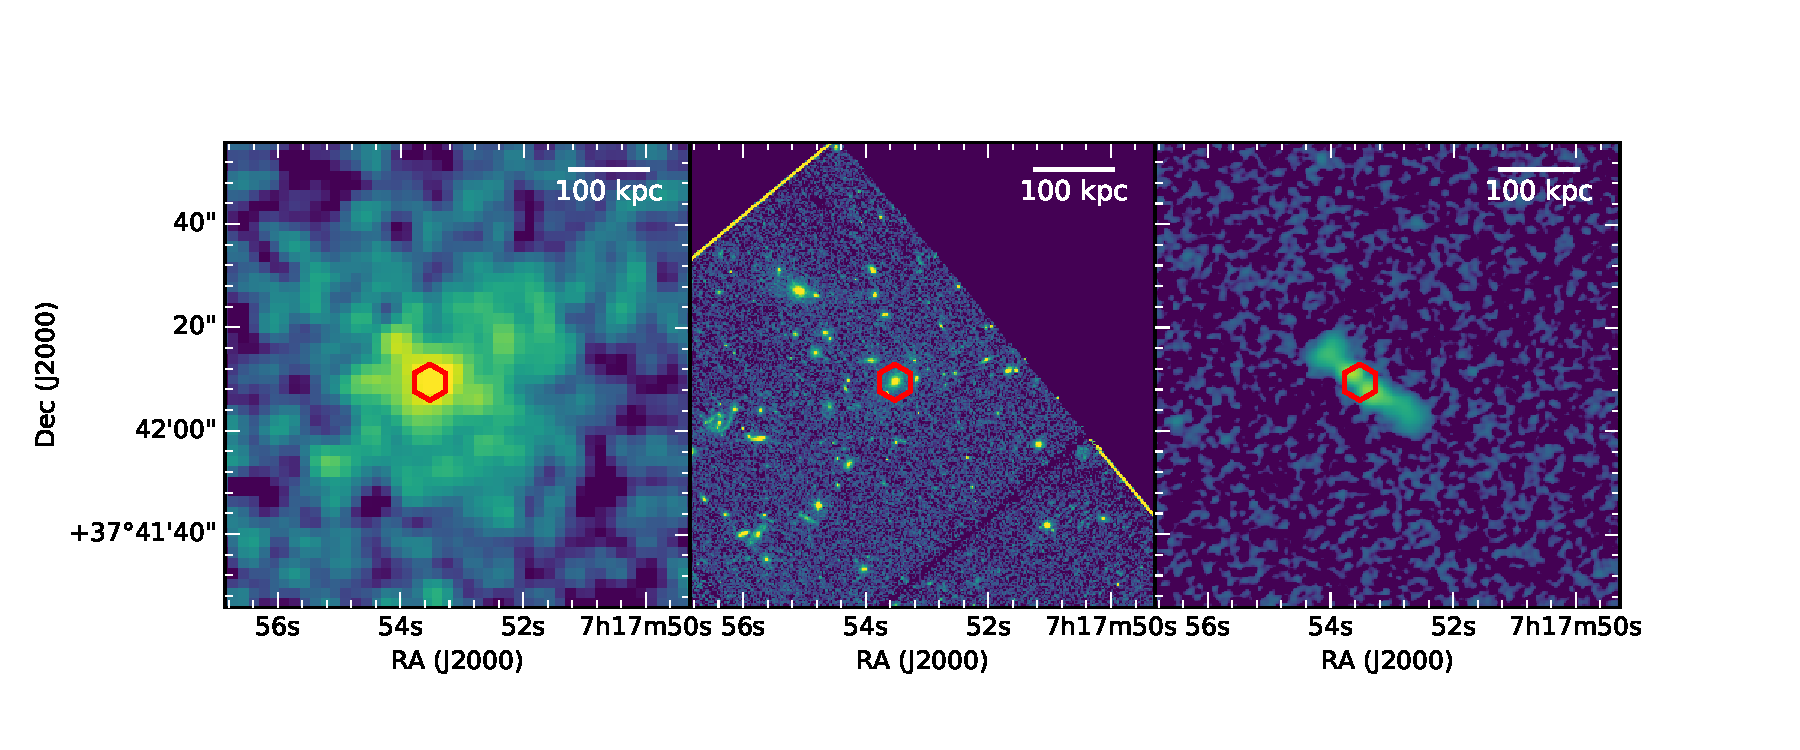
\includegraphics[width=\textwidth]{plots/group_bcg.pdf}
	\caption{$0.5-4$~keV  \chandra\ (left), F606W \emph{HST} (middle; PropID 10084), and $1-2$~GHz L-band A-array \emph{VLA} (right) images of the region occupied by the galaxy group in the filament. The red hexagon marks the position of the group's centrally dominant galaxy (BCG). The size of the radio beam (10.7~kpc~$\times$~9.0 kpc) is shown in the bottom left corner of the radio image. Results from the radio data are described by van Weeren et al., submitted. The position of the BCG coincides with those of the radio AGN and of the X-ray peak.\label{fig:group}}
\end{figure*}

The group of galaxies within the large-scale filament is located in projection a little over 2~Mpc SE of the cluster center, fixed at ${\rm RA} = 07^{\rm h}\, 17^{\rm m}\, 30.025^{\rm s}$, ${\rm Dec} = +37^{\circ}\, 45\arcmin \, 18.58\arcmin\arcmin$ for consistency with \citet{Jauzac2012}. The small size of the group and its large distance from the cluster implies that it is falling for the first time towards MACS~J0717.5+3745, rather than having traversed the cluster from the NW to the SE. This interpretation is also supported by the fact that the position of the X-ray peak is consistent with those of the cD galaxy and of the AGN hosted by the galaxy, as seen in Figure~\ref{fig:group}.

We measured the temperature and the brightness of the group by extracting spectra within $r_{\rm 2500} \approx 300$~kpc \citep{Medezinski2013}. The circular region, shown in Figure~\ref{fig:fil}, had the center fixed at ${\rm RA} = 07^{\rm h}\, 17^{\rm m}\, 53.347^{\rm s}$, ${\rm Dec} = +37^{\circ}\, 42\arcmin \, 09.25\arcmin\arcmin$. We assumed a group metallicity of 0.2 solar \citep[e.g.,][]{Rasmussen2007}. The best-fitting parameters are summarized in Table~\ref{tab:spectra}. The cluster has a $r_{2500}$ temperature of $4.19_{-0.48}^{+0.76}$~keV. The normalization is equivalent to a bolometric luminosity of $(1.2\pm 0.1) \times 10^{44}$~erg~s$^{-1}$. Based on the luminosity-mass scaling relations for galaxy groups \citep[e.g.,][]{Connor2014}, the group's luminosity corresponds to $M_{\rm 2500} \sim 6-7\times 10^{13}$~M$_\odot$. A consistent mass estimate is obtained from the temperature-mass scaling relations.  Using optical data, \citet{Medezinski2013} determined $M_{\rm 2500} = (7.4\pm 3.0) \times 10^{13}$~M$_\odot$, which is also consistent with our estimate. The group thus sits on the luminosity-mass and temperature-mass relations, which is further indication that no significant stripping by the cluster has occurred yet.

\section{X-ray Emission from the Filament}
\label{sec:Filament}

\begin{figure*}
    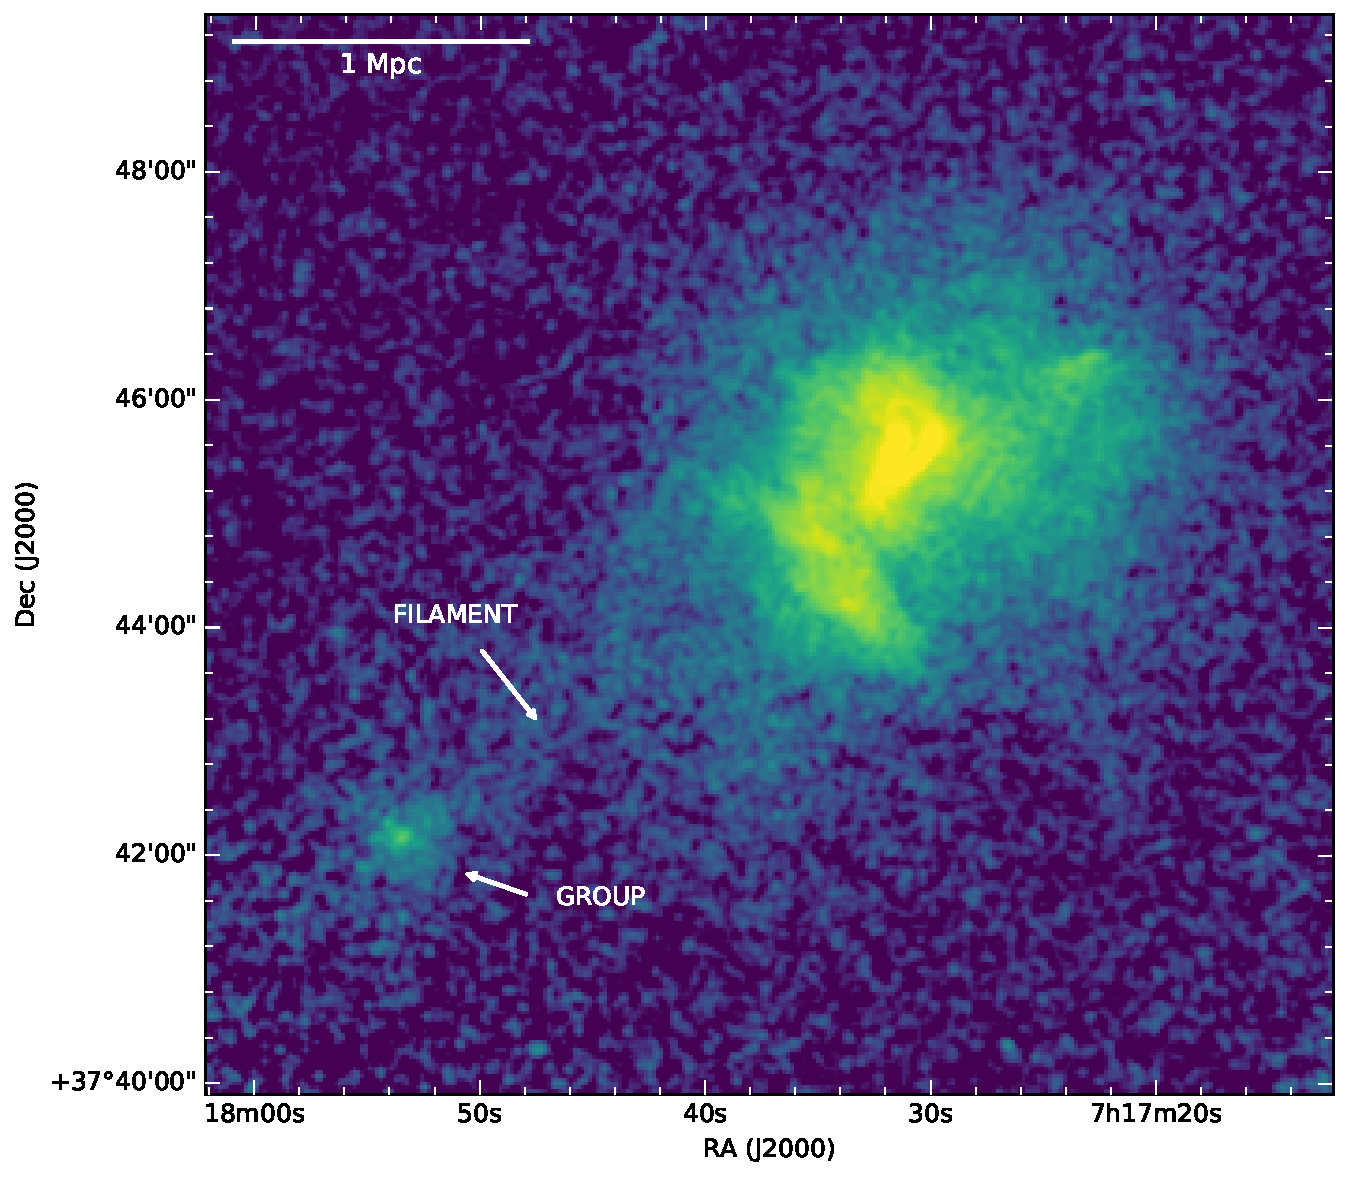
\includegraphics[width=\columnwidth]{plots/fil-labels.pdf}
    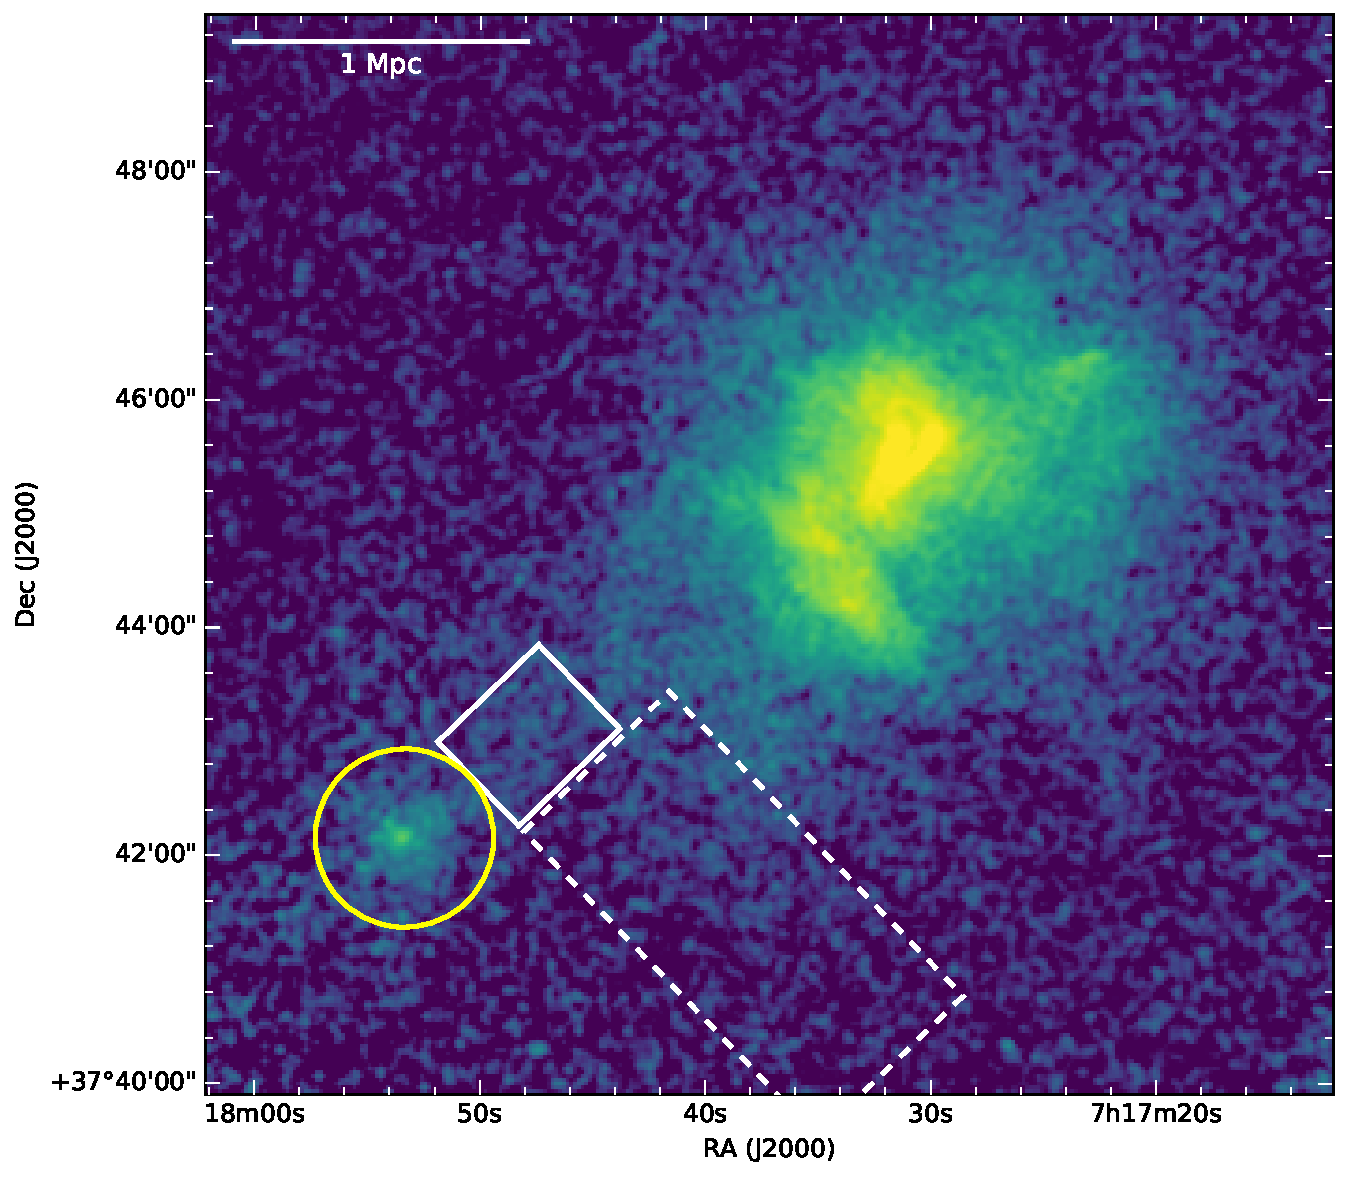
\includegraphics[width=\columnwidth]{plots/fil-regions.pdf}
    \caption{\emph{Left:} Chandra $0.5-4$~keV surface brightness map of MACS J0717.5+3745, showing the features discussed in this work. The image was exposure- and vignetting-corrected. Point sources were subtracted and the gaps were filled by sampling the regions surrounding the point sources. The gaps were filled to create a more visually appealing figure. However, the imaging analysis was done on images that did not have the gaps filled. The images used in the analysis are available online as supporting material. \emph{Right:} Regions used in the spectral analysis. The regions of main interest are drawn in solid lines, while the regions used to characterize the contaminating/surrounding emission are drawn in dashed lines. The best-fitting parameters obtained for the gas in these regions are listed in Table~\ref{tab:spectra}. \label{fig:fil}}
\end{figure*}

\begin{table}
  \caption{Parameters of the regions used for the spectral analysis. The regions are shown in Figure~\ref{fig:fil}. Uncertainties are quoted at the $\Delta C = 1$ level. \label{tab:spectra}}
  \begin{center}
    \begin{threeparttable}
      \begin{tabular}{l c c}
              \multicolumn{3}{c}{\textsc{Foreground and Background}} \\
              \hline\hline
              Model Component & Temperature\tnote{a} & Normalization\tnote{b} \\
              \hline
              Local Hot Bubble & $0.135_{-0.008}^{+0.007}$ & $7.21_{-0.18}^{+0.30} \times 10^{-7}$ \\
              Galactic Halo & $0.59_{-0.08}^{+0.09}$ & $2.78_{-0.44}^{+0.45} \times 10^{-7}$ \\
              Unresolved Background       &\multirow{2}{*}{ -- } & \multirow{2}{*}{ $4.44_{-0.37}^{+0.35} \times 10^{-7}$} \\
              Sources ObsID 16235/16305 &                                    &            \\
              Unresolved Background       &\multirow{2}{*}{ -- } & \multirow{2}{*}{ $7.02_{-0.58}^{+0.49} \times 10^{-7}$} \\
              Sources ObsID 4200               &                                    &            \\
              \multicolumn{3}{c}{} \\
              \multicolumn{3}{c}{\textsc{Large-Scale Filament}} \\
              \hline\hline
                Region & Temperature\tnote{a} & Normalization\tnote{b} \\
              \hline
               A using B & $1.58_{-0.25}^{+0.51}$ & $4.00_{-0.60}^{+0.56} \times 10^{-5}$ \\
               A using C & $1.54_{-0.25}^{+0.50}$ & $3.78_{-0.52}^{+0.55} \times 10^{-5}$ \\
               C & $8.90_{-1.65}^{+4.25}$ & $1.70_{-0.08}^{+0.09} \times 10^{-5}$  \\
               B & $11.55_{-3.95}^{+9.09}$ & $1.55_{-0.10}^{+0.14} \times 10^{-5}$  \\
              \multicolumn{3}{c}{} \\
              \multicolumn{3}{c}{\textsc{Group in the Filament}} \\
              \hline\hline
                             & Temperature\tnote{a} & Normalization\tnote{b} \\
              \hline
                            & $4.19_{-0.48}^{+0.76}$ & $ 8.40_{-0.53}^{+0.52} \times 10^{-5}$ \\
              \multicolumn{3}{c}{} \\
              \multicolumn{3}{c}{\textsc{ `Finger' (Region D)}} \\
              \hline\hline
                             & Temperature\tnote{a} & Normalization\tnote{b} \\
              \hline
                            & $1.55_{-0.52}^{+1.67}$ & $ 1.57_{-0.44}^{+0.32} \times 10^{-5}$ \\
      \end{tabular}
      \begin{tablenotes}
              \item[a] Units of keV.
              \item[b] Units of cm$^{-5}$~arcmin$^{-2}$ for the thermal components, and photons~keV$^{-1}$~cm$^{-2}$~s$^{-1}$~arcmin$^{-2}$ at 1~keV for the power-law components.
      \end{tablenotes}
    \end{threeparttable}
  \end{center}
\end{table}

To define the region of the filament that is least contaminated by ICM emission, we examined the surface brightness profile in a rectangular region aligned with the filament. In this region, the surface brightness decreases away from the cluster center, and then increases again approaching the SE group located along the filament; there is no radial range in this region where the surface brightness is flat. This suggests that the ICM of MACS~J0717.5+3745 contaminates the filament, and this contamination needs to be considered when modeling the filament emission. Alternatively, the intrinsic brightness of the filament would be decreasing towards the group; however, evidence for this scenario is weak, especially given that faint ICM emission is seen SW of the filament.

We modeled the filament and the ``contamination'' from the ICM by extracting spectra in three regions: a rectangular region centered on the filament (A), another rectangular region positioned to its SW (B), and a NW partial annulus on the side of the cluster opposite to the filament (C). The latter region is at the same distance from the cluster center as the filament region. Regions B and C are used separately to model ICM contamination. All the regions are shown in Figure~\ref{fig:fil}. 

We excluded the ICM regions NE and SW of the cluster center for the analysis of the filament properties. NE of the filament region and NE of the cluster center, the signal-to-noise is too low for any meaningful information to be extracted from the spectrum. SW of the cluster center, most of the photons originate from an isolated `finger'-shaped cold region (D) with temperatures of $\sim 2$~keV. This region is discussed in the next section. 

The emission in regions B and C was modeled with single thermal components, while the emission in the filament region (A) was modeled with two thermal components--one describing ICM contamination, whose parameters were successively linked to those of the thermal component used to describe regions B/C, and one describing emission from the filament. The thermal components were modeled with APEC models. We performed two fits: one in which the spectra from regions A and B were fitted simultaneously (ignoring the spectrum from region C), and one in which the spectra from regions A and C were fitted simultaneously (ignoring the spectrum from region B). Table~\ref{tab:spectra} lists the best-fitting parameters obtained for a fixed gas metallicity of 0.2 solar. Typical metallicities of cosmic filaments are still an open question, and it is plausible that they are lower than the typical metallicities in the outskirts of galaxy clusters \citep[$\sim 0.2-0.3$ solar; e.g.][]{Simionescu2015}. In this case, varying the metallicity causes only minor changes to the best-fitting parameters, well within the statistical uncertainty ranges. In one of the \textsc{Jupyter} notebooks supporting this paper, we also list results obtained for metallicities of 0 and 0.1 solar.\footnote{\url{https://goo.gl/7x2pXR}}

The \textsc{XSpec} normalizations of the thermal components listed in Table~\ref{tab:spectra} are defined as
\begin{equation}
	\mathcal{N} = \frac{n_{\rm e} \, n_{\rm H} \, V}{10^{14} \, 4\pi \, S_{\rm reg} \, D_{\rm A}^2 \, (1+z)^2} \, , 
\label{eq:norm}
\end{equation}
where we assume the density to be constant in each region, where $n_{\rm e}$ is the electron number density, $n_{\rm H}$ is the hydrogen number density, $V$ is the volume of the region, $S_{\rm reg}$ is the projected area of the region, $D_{\rm A}$ is the angular size distance to the cluster, and $z$ is the cluster redshift.

\begin{figure}
	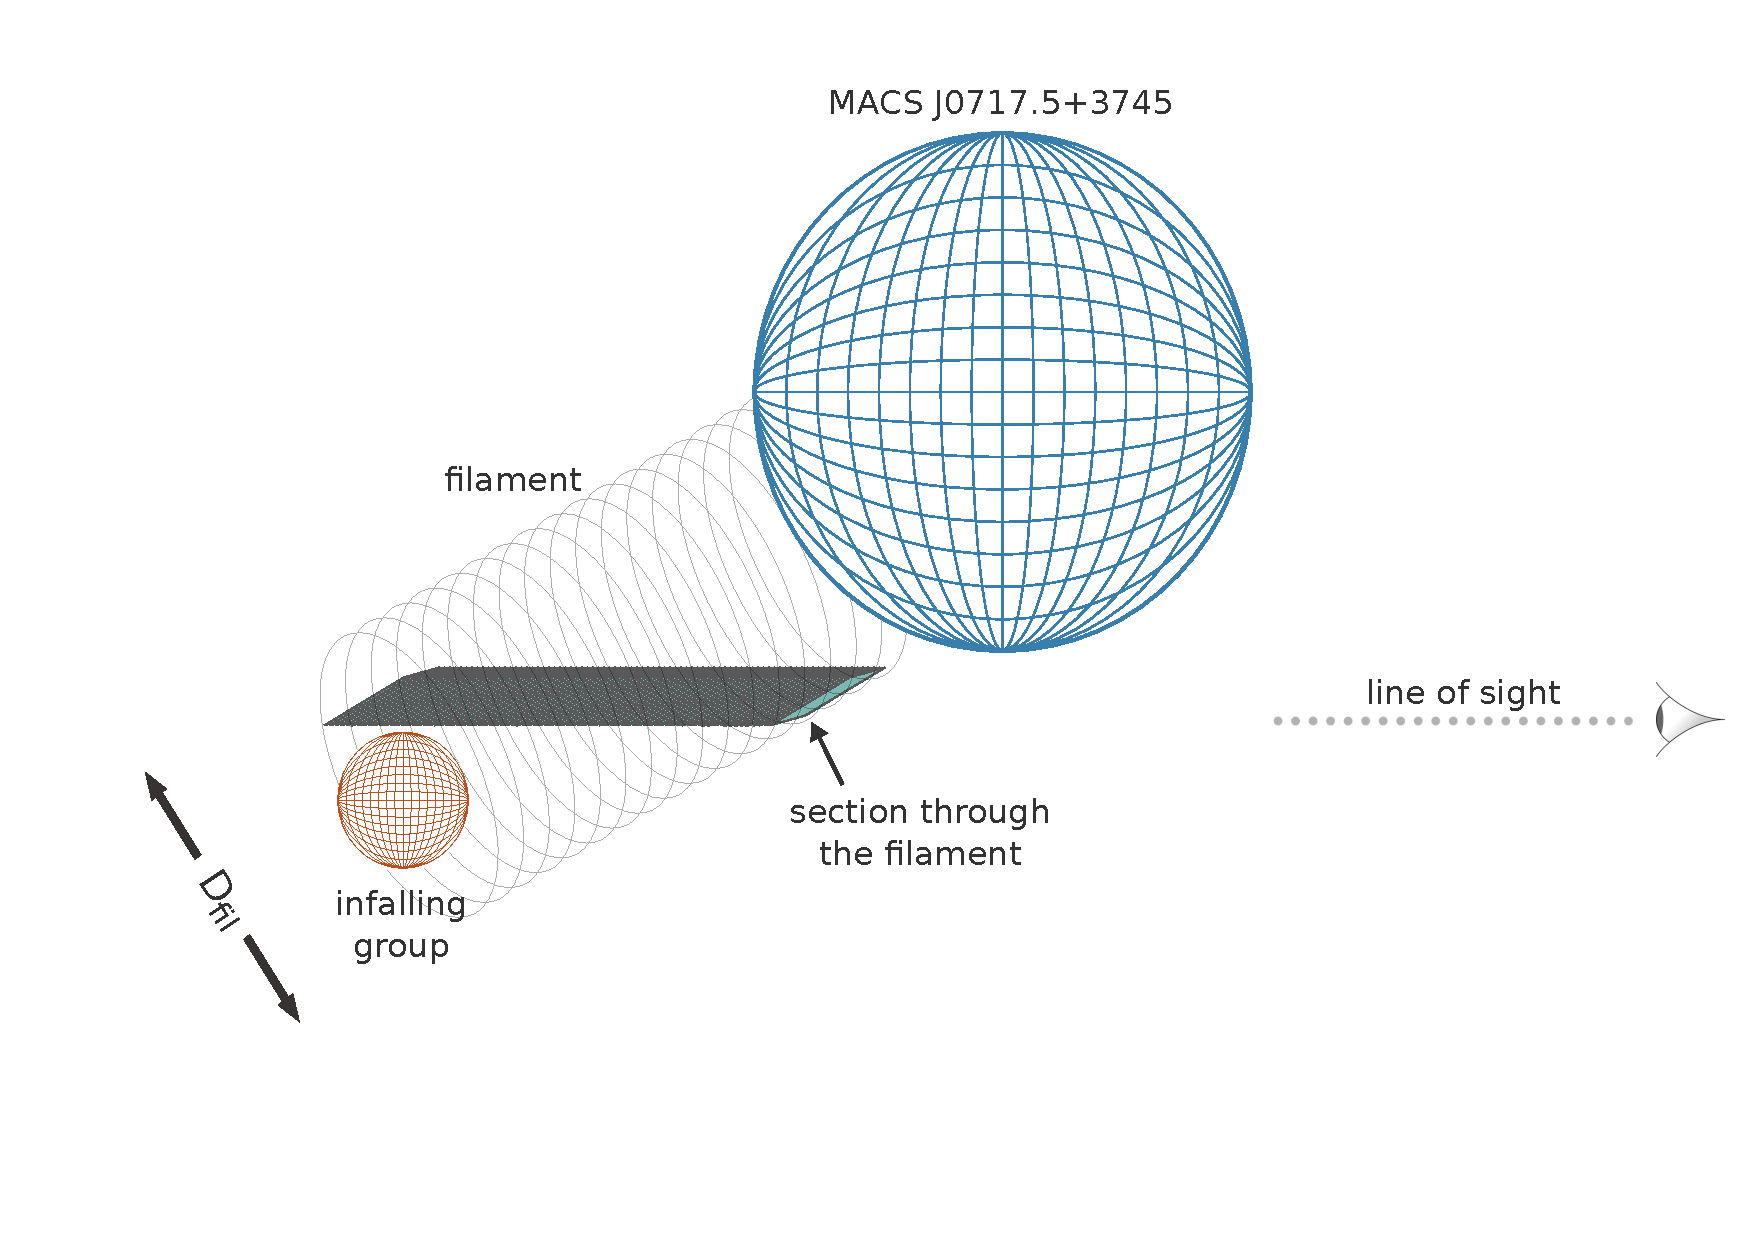
\includegraphics[width=\columnwidth, trim=0 2.5cm 0 1cm, clip=True]{plots/fil-macsj0717-sketch.pdf}
	\caption{Sketch illustrating the geometry assumed for the large scale filament. The results vary insignificantly (compared to our other uncertainties) when assuming a parallelepiped geometry instead of a more natural cylindrical shape. For simplicity, we therefore used a parallelepiped for our volume estimate. The parallelepiped has two rectangular faces perpendicular to the line of sight, and two rectangular and two parallelogram faces parallel to the line of sight. The normal to the parallelogram faces points perpendicular to the page.  \label{fig:sketch}}
\end{figure}

To estimate the density in the filament, we treat it as a cylinder with its axis inclined to the plane of the sky. \citet{Jauzac2012}, citing Ebeling et al., in prep., assume that the inclination angle between the filament axis and the plane of the sky is $\theta \sim 75$~degrees. We adopt this value here, noting that it is highly uncertain and the results below are sensitive to it. \citet{Jauzac2012} also determined the diameter of the filament to be $D_{\rm fil} \sim 3$~Mpc at the position where our spectra were extracted. Approximating the 3D region within the filament projected onto our spectral region as a parallelepiped (Fig.~\ref{fig:sketch}), its volume is 
\begin{eqnarray}
    V \equiv V_{\rm ppp} = D_{\rm fil} \; S_{\rm reg} / \cos\theta\,  . 
\label{eq:v_ppp}
\end{eqnarray}

The projected region has a length of $1.2$~arcmin ($\approx 460$~kpc) and a width of $1$~arcmin ($\approx 380$~kpc), therefore $S_{\rm reg} = 1.2$~arcmin$^{2}$. Assuming $n_{\rm e} = 1.2\, n_{\rm H}$ \citep[e.g.,][]{Bohringer2010}, and finally substituting Eq.~\ref{eq:v_ppp} in Eq.~\ref{eq:norm}, the electron number density in the X-ray bright part of the filament is $\sim 2\times 10^{-4}$~cm$^{-3}$. The critical density of the Universe at the redshift of MACS~J0717.5+3745 is $1.7\times 10^{-29}$~g~cm$^{-3}$. Assuming the total baryon density is $4.4\%$ the critical density of the Universe \citep{Kirkman2003}, the filament is overdense by a factor of $\sim 450$ compared to the mean baryon density of the Universe. Assuming a baryon mass fraction of $0.15$ \citep[e.g.,][]{Mantz2014} within the filament, the mass density of the filament is $\sim 3\times 10^{13}$~M$_{\odot}$~Mpc$^{-3}$. The filament density is in excellent agreement with the density calculated from the weak lensing data by \citet{Jauzac2012} for the same filament geometry. The filament density corresponds to an overdensity of $\sim 100-150$ relative to the critical density of the Universe.\footnote{\citet{Jauzac2012} calculate an overdensity of $206\pm 46$~$\rho_{\rm crit}$, about $65\%$ higher than our value, but this appears to be due to a mistake in the density conversion; our filament mass density values are consistent.} 

The X-ray emission from the brightest part of the filament could originate from the hottest gas phase of the WHIM. Its density and temperature are consistent with reports of WHIM X-ray detection from other cluster filaments \citep[e.g.,][]{Werner2008, Eckert2015}. Alternatively, at least part of the X-ray emission could be due to gas stripped from substructure that fell onto the cluster along the large-scale filament \citep[similarly to what is seen in A85;][]{Ichinohe2015}. However, the latter interpretation requires that the X-ray-bright part of the filament is within the virial radius of MACS~J0717.5+3745 \citep[$r_{\rm 138} = 2.5$~Mpc;][]{Medezinski2013}, which would imply a filament inclination angle of $\lesssim 60^\circ$. 

For the densities calculated above, the mass of the filament in the region from which the spectra were extracted is $\sim 6\times 10^{13}$~M$_\odot$, with $\sim 9\times 10^{12}$~M$_\odot$ in the hot gas. 

\begin{figure*}
   \renewcommand{\arraystretch}{1.5}
    \begin{tabular}{m{\columnwidth}m{0.9\columnwidth}}
    \multicolumn{2}{l}{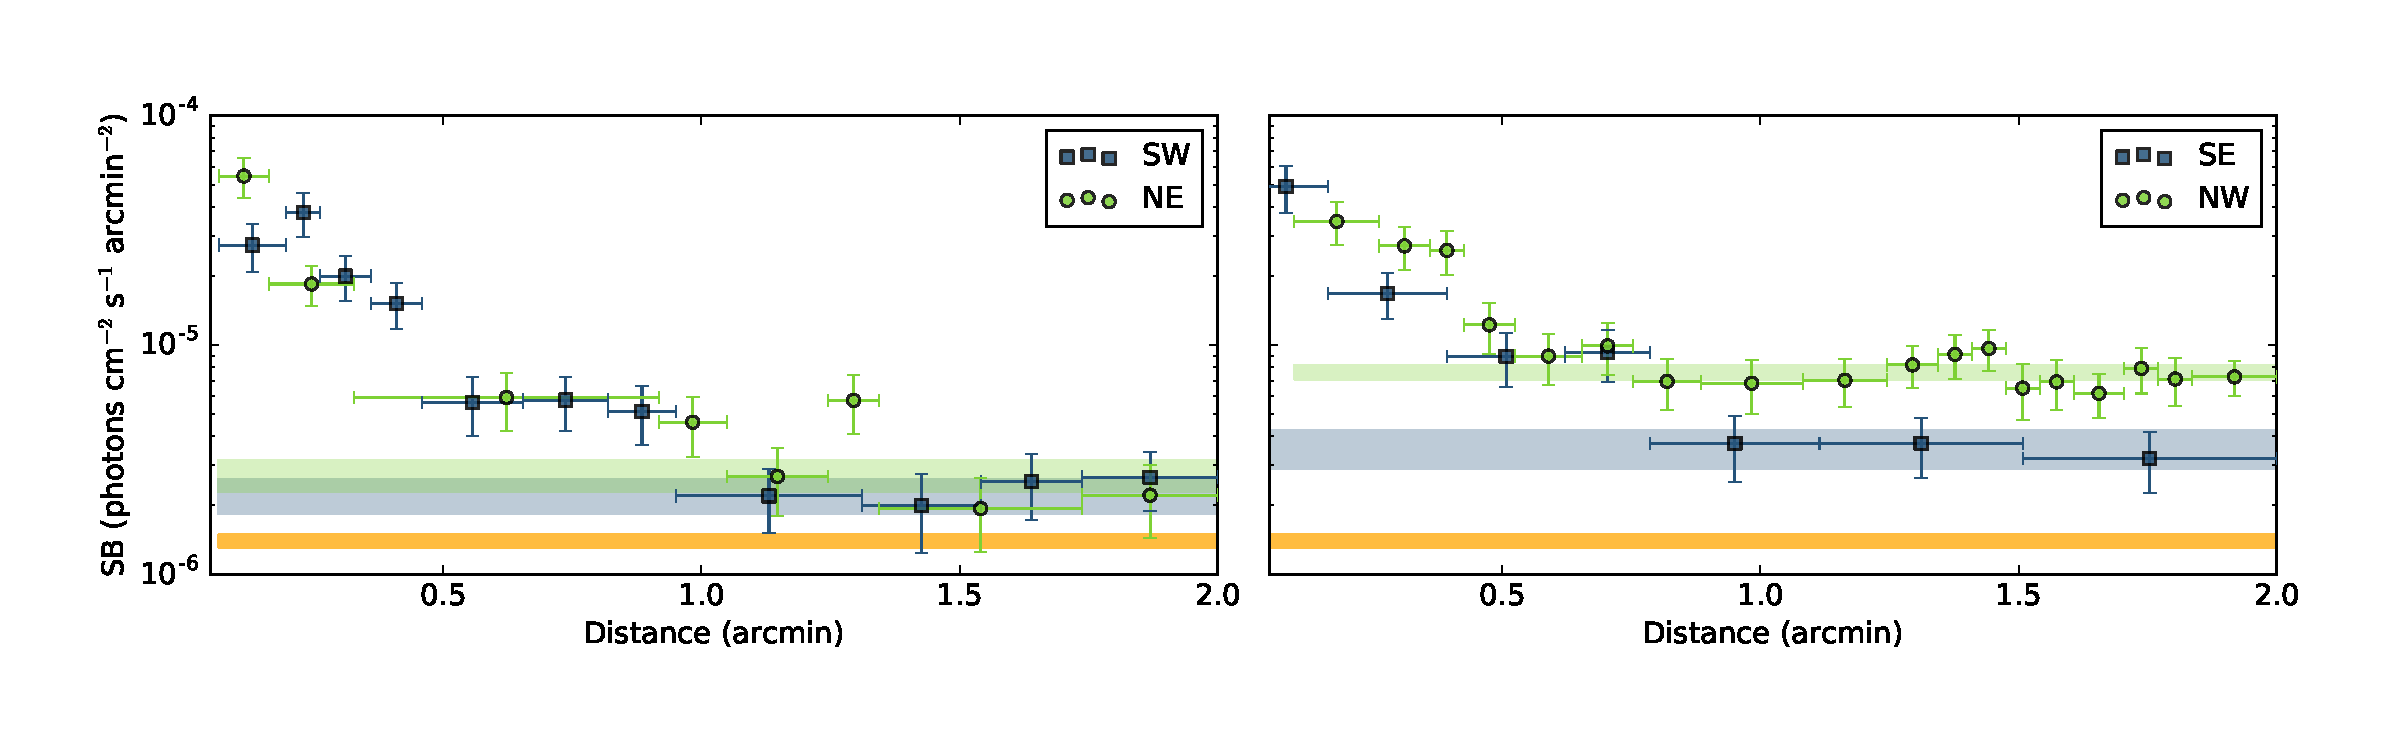
\includegraphics[width=\textwidth]{plots/macsj0717-group-all-directions.pdf}} \vspace{-0.5cm} \\
    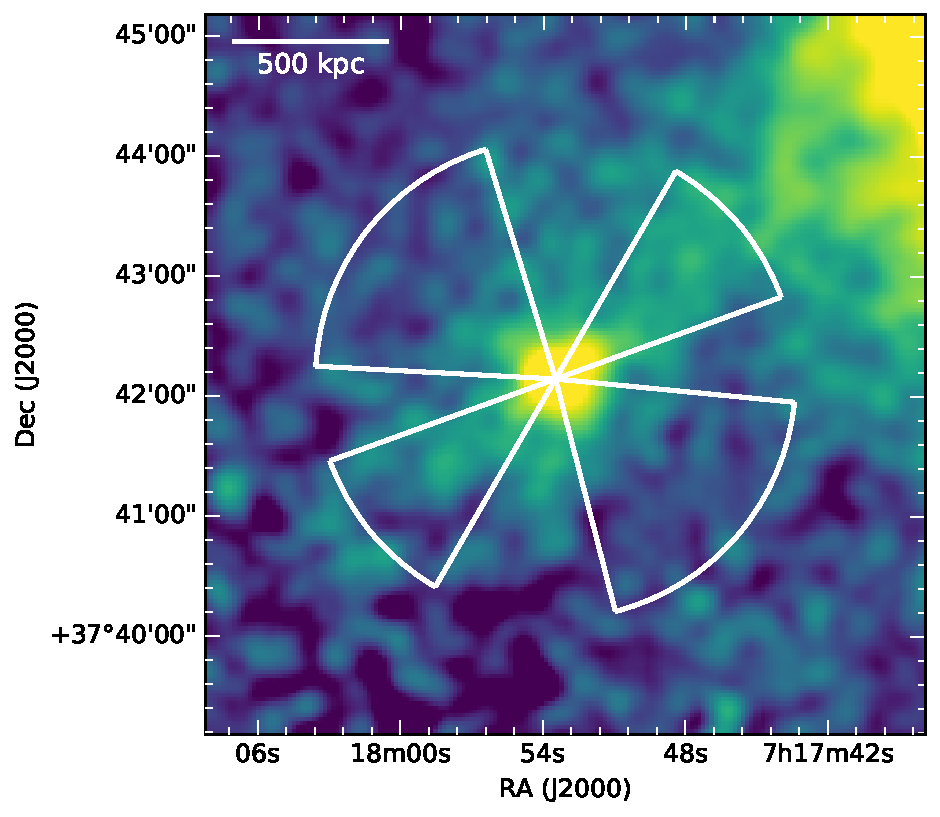
\includegraphics[width=\columnwidth]{plots/group-sectors.pdf}
    & \hspace{0.15cm}\multicolumn{1}{b{0.85\columnwidth}}{\caption{\emph{Top:} Surface brightness profiles perpendicular to (left) and along (right) the filament. The light-colored green and blue bands show the average surface brightness between 1 and 2 arcmin, where the emission from the group is negligible. The orange band shows the $1\sigma$ confidence range of the sky background level. \emph{Bottom:} Sectors from which the surface brightness profiles shown above were extracted. The sectors are centered on the X-ray peak of the galaxy group. }} 
    \label{fig:group-sx}
    \end{tabular}
\end{figure*}

In Figure~\ref{fig:group-sx}, we show the surface brightness profiles in four sectors centered on the galaxy group seen within the filament. The surface brightness of the group becomes negligible beyond 1 arcmin. Between 1 and 2 arcmin, the profiles show the NW sector being significantly brighter than the other three; this sector covers the part of the filament between the group and the cluster. On the other side of the group, in the SE sector, the surface brightness between 1 and 2 arcmin is also larger than in the directions perpendicular to the filament. The SE sector includes part of the filament at higher cluster-centric radii. The surface brightness here is about half of that in the NW sector, which implies a baryon density lower by a factor of $\sim 1.5$ compared to the part of the filament closer to the cluster if the diameter of the filament is the same on both sides of the group. However, \citet{Jauzac2012} found that the diameter of the filament might be decreasing by a factor of up to $\sim 2$ from the region ahead of the group to the region beyond the group. Bearing in mind that the filament diameter measurements of \citet{Jauzac2012} are highly uncertain, a decrease in diameter could account for the difference in surface brightness.

The calculations made above can be found in one of the supporting \textsc{Jupyter} notebooks accompanying this paper.\footnote{\url{https://goo.gl/7x2pXR}}

\section{`Finger' of Cool Emission}
\label{sec:finger}

Extending SW of the cluster center, roughly at the same cluster-centric distance as the X-ray-bright section of the filament (A), there is a `finger' of X-ray emission. This feature is labeled in Figure~\ref{fig:fil} as region~D. NW and SE of the `finger', at the same cluster-centric distance, the signal-to-noise ratio is essentially zero. This suggests that contamination from the cluster ICM is minimal in the `finger', and therefore we modeled the emission in region~D with a single thermal component. The temperature of the gas in the `finger' is $\sim 1-3$~keV, comparable to the temperature of the gas in region A of the filament.

The `finger' could be the X-ray-bright part of another large-scale cosmic filament, or cold gas stripped from one of the merging clusters that was not yet heated up. Narrowing down on the origin of the `finger' would require knowledge about its inclination angle with respect to the plane of the sky in order to determine its distance from the cluster center. If the `finger' is within the cluster's virial radius, then it would be unheated gas from one of the merging clusters. Alternatively, if the `finger' is outside the cluster's virial radius, we would interpret it as being part of a cosmic filament. 


\section{Summary}
\label{sec:Summary}

MACS~J0717.5+3745 ($z=0.546$) is one of the six massive Frontier Fields clusters. The cluster is the most morphologically complex merger, being the site of collisions between at least four subclusters. SE of the cluster, there is a large-scale cosmic filament that was first reported by \citet{Ebeling2004}. Some of the subclusters involved in the merger have likely traveled along this filament before colliding with the previously existing structure. \citet{Jauzac2012} determined from optical data that the filament is $\sim 19$~Mpc long. The part of the filament that is near the cluster is visible at X-ray wavelengths. So far, the thermodynamic properties of large-scale filaments have only been studied in a handful of merging clusters \citep{Werner2008, Eckert2015, Bulbul2016}. Here, we used deep \chandra\ observations of MACS~J0717.5+3745 to study the properties of the large-scale filament extending SE of the cluster center, and those of the substructures along the filament. Below is a summary of our results:

\begin{itemize}
	\item The filament has a temperature of $1.58_{-0.25}^{+0.51}$~keV and a density of $\sim 10^{-4}$ cm$^{-3}$. These are consistent at the $90\%$ confidence level with the properties of the other filaments studied in X-rays \citep{Werner2008, Eckert2015, Bulbul2016}.
	\item The filament is over-dense by a factor of $\sim 100-150$ compared to the critical density of the Universe at the cluster redshift.
	\item The X-ray emission from the filament could be coming from the hottest and densest gas of the WHIM, or (at least partly) from gas stripped from substructures that fell into the cluster along the large-scale filament.
	\item The total mass contained in the X-ray-bright region of the filament is $\sim 6\times 10^{13}$~M$_\odot$, with $\sim 9\times 10^{12}$~M$_\odot$ in the hot gas.
	\item A little over $2$~Mpc SE of the cluster center, embedded within the filament, there is a galaxy group with a temperature of $\sim 4$~keV and an X-ray bolometric luminosity of $\sim 10^{44}$~erg~s$^{-1}$. The mass of the group is estimated to be $\sim 6-7\times 10^{13}$~M$_\odot$. This group is likely approaching the cluster for the first time.
\end{itemize}

\acknowledgments
GAO acknowledges support by NASA through a Hubble Fellowship grant HST-HF2-51345.001-A awarded by the Space Telescope Science Institute, which is operated by the Association of Universities for Research in Astronomy, Incorporated, under NASA contract NAS5-26555. RJvW is supported by a Clay Fellowship awarded by the Harvard-Smithsonian Center for Astrophysics. FAS acknowledges support from \chandra\ grant GO3-14131X.

This research made use of \textsc{APLpy}, an open-source plotting package for \textsc{Python} hosted at \url{http://aplpy.github.com}, and of \textsc{Astropy}, a community-developed core \textsc{Python} package
  for Astronomy \citep{astropy}. This research has also made use of NASA's Astrophysics Data System, and of the cosmology calculator developed by N. Wright \citep{Wright2006}. The \chandra\ data was obtained from the Chandra Data Archive, and analyzed using software provided by the Chandra X-ray Center (CXC) in the application packages \textsc{CIAO} and \textsc{ChIPS}. The X-ray surface brightness profiles were created with \textsc{PyXel} (available at \url{https://github.com/gogrean/pyxel}) and plotted using \textsc{matplotlib}, a \textsc{Python} library for publication quality graphics \citep{Hunter2007}.
  
 The optical data shown in the paper is based on observations made with the NASA/ESA Hubble Space Telescope, and obtained from the \href{http://hla.stsci.edu/}{Hubble Legacy Archive}, which is a collaboration between the Space Telescope Science Institute (STScI/NASA), the Space Telescope European Coordinating Facility (ST-ECF/ESA) and the Canadian Astronomy Data Centre (CADC/NRC/CSA).

\begin{thebibliography}{34}
\expandafter\ifx\csname natexlab\endcsname\relax\def\natexlab#1{#1}\fi

\bibitem[{{Astropy Collaboration} {et~al.}(2013){Astropy Collaboration},
  {Robitaille}, {Tollerud}, {Greenfield}, {Droettboom}, {Bray}, {Aldcroft},
  {Davis}, {Ginsburg}, {Price-Whelan}, {Kerzendorf}, {Conley}, {Crighton},
  {Barbary}, {Muna}, {Ferguson}, {Grollier}, {Parikh}, {Nair}, {Unther},
  {Deil}, {Woillez}, {Conseil}, {Kramer}, {Turner}, {Singer}, {Fox}, {Weaver},
  {Zabalza}, {Edwards}, {Azalee Bostroem}, {Burke}, {Casey}, {Crawford},
  {Dencheva}, {Ely}, {Jenness}, {Labrie}, {Lim}, {Pierfederici}, {Pontzen},
  {Ptak}, {Refsdal}, {Servillat}, \& {Streicher}}]{astropy}
{Astropy Collaboration}, {Robitaille}, T.~P., {Tollerud}, E.~J., {et~al.} 2013,
  \aap, 558, A33

\bibitem[{{B{\"o}hringer} \& {Werner}(2010)}]{Bohringer2010}
{B{\"o}hringer}, H., \& {Werner}, N. 2010, \aapr, 18, 127

\bibitem[{{Bulbul} {et~al.}(2016){Bulbul}, {Randall}, {Bayliss}, {Miller},
  {Andrade-Santos}, {Johnson}, {Bautz}, {Blanton}, {Forman}, {Jones},
  {Paterno-Mahler}, {Murray}, {Sarazin}, {Smith}, \& {Ezer}}]{Bulbul2016}
{Bulbul}, E., {Randall}, S.~W., {Bayliss}, M., {et~al.} 2016, \apj, 818, 131

\bibitem[{{Connor} {et~al.}(2014){Connor}, {Donahue}, {Sun}, {Hoekstra},
  {Mahdavi}, {Conselice}, \& {McNamara}}]{Connor2014}
{Connor}, T., {Donahue}, M., {Sun}, M., {et~al.} 2014, \apj, 794, 48

\bibitem[{{Dav{\'e}} {et~al.}(2001){Dav{\'e}}, {Cen}, {Ostriker}, {Bryan},
  {Hernquist}, {Katz}, {Weinberg}, {Norman}, \& {O'Shea}}]{Dave2001}
{Dav{\'e}}, R., {Cen}, R., {Ostriker}, J.~P., {et~al.} 2001, \apj, 552, 473

\bibitem[{{Dietrich} {et~al.}(2005){Dietrich}, {Schneider}, {Clowe},
  {Romano-D{\'{\i}}az}, \& {Kerp}}]{Dietrich2005}
{Dietrich}, J.~P., {Schneider}, P., {Clowe}, D., {Romano-D{\'{\i}}az}, E., \&
  {Kerp}, J. 2005, \aap, 440, 453

\bibitem[{{Dietrich} {et~al.}(2012){Dietrich}, {Werner}, {Clowe}, {Finoguenov},
  {Kitching}, {Miller}, \& {Simionescu}}]{Dietrich2012}
{Dietrich}, J.~P., {Werner}, N., {Clowe}, D., {et~al.} 2012, \nat, 487, 202

\bibitem[{{Ebeling} {et~al.}(2004){Ebeling}, {Barrett}, \&
  {Donovan}}]{Ebeling2004}
{Ebeling}, H., {Barrett}, E., \& {Donovan}, D. 2004, \apjl, 609, L49

\bibitem[{{Ebeling} {et~al.}(2007){Ebeling}, {Barrett}, {Donovan}, {Ma},
  {Edge}, \& {van Speybroeck}}]{Ebeling2007}
{Ebeling}, H., {Barrett}, E., {Donovan}, D., {et~al.} 2007, \apjl, 661, L33

\bibitem[{{Ebeling} {et~al.}(2001){Ebeling}, {Edge}, \& {Henry}}]{Ebeling2001}
{Ebeling}, H., {Edge}, A.~C., \& {Henry}, J.~P. 2001, \apj, 553, 668

\bibitem[{{Eckert} {et~al.}(2015){Eckert}, {Jauzac}, {Shan}, {Kneib}, {Erben},
  {Israel}, {Jullo}, {Klein}, {Massey}, {Richard}, \& {Tchernin}}]{Eckert2015}
{Eckert}, D., {Jauzac}, M., {Shan}, H., {et~al.} 2015, \nat, 528, 105

\bibitem[{{Einasto} {et~al.}(1994){Einasto}, {Einasto}, {Tago}, {Dalton}, \&
  {Andernach}}]{Einasto1994}
{Einasto}, M., {Einasto}, J., {Tago}, E., {Dalton}, G.~B., \& {Andernach}, H.
  1994, \mnras, 269, 301

\bibitem[{{Elvis} {et~al.}(1992){Elvis}, {Plummer}, {Schachter}, \&
  {Fabbiano}}]{Elvis1992}
{Elvis}, M., {Plummer}, D., {Schachter}, J., \& {Fabbiano}, G. 1992, \apjs, 80,
  257

\bibitem[{{Feldman}(1992)}]{Feldman1992}
{Feldman}, U. 1992, \physscr, 46, 202

\bibitem[{Hunter(2007)}]{Hunter2007}
Hunter, J.~D. 2007, Computing In Science \& Engineering, 9, 90

\bibitem[{{Ichinohe} {et~al.}(2015){Ichinohe}, {Werner}, {Simionescu}, {Allen},
  {Canning}, {Ehlert}, {Mernier}, \& {Takahashi}}]{Ichinohe2015}
{Ichinohe}, Y., {Werner}, N., {Simionescu}, A., {et~al.} 2015, \mnras, 448,
  2971

\bibitem[{{Jauzac} {et~al.}(2012){Jauzac}, {Jullo}, {Kneib}, {Ebeling},
  {Leauthaud}, {Ma}, {Limousin}, {Massey}, \& {Richard}}]{Jauzac2012}
{Jauzac}, M., {Jullo}, E., {Kneib}, J.-P., {et~al.} 2012, \mnras, 426, 3369

\bibitem[{{Kalberla} {et~al.}(2005){Kalberla}, {Burton}, {Hartmann}, {Arnal},
  {Bajaja}, {Morras}, \& {P{\"o}ppel}}]{Kalberla2005}
{Kalberla}, P.~M.~W., {Burton}, W.~B., {Hartmann}, D., {et~al.} 2005, \aap,
  440, 775

\bibitem[{{Kirkman} {et~al.}(2003){Kirkman}, {Tytler}, {Suzuki}, {O'Meara}, \&
  {Lubin}}]{Kirkman2003}
{Kirkman}, D., {Tytler}, D., {Suzuki}, N., {O'Meara}, J.~M., \& {Lubin}, D.
  2003, \apjs, 149, 1

\bibitem[{{Ma} {et~al.}(2009){Ma}, {Ebeling}, \& {Barrett}}]{Ma2009}
{Ma}, C.-J., {Ebeling}, H., \& {Barrett}, E. 2009, \apjl, 693, L56

\bibitem[{{Mantz} {et~al.}(2014){Mantz}, {Allen}, {Morris}, {Rapetti},
  {Applegate}, {Kelly}, {von der Linden}, \& {Schmidt}}]{Mantz2014}
{Mantz}, A.~B., {Allen}, S.~W., {Morris}, R.~G., {et~al.} 2014, \mnras, 440,
  2077

\bibitem[{{Markevitch} {et~al.}(2002){Markevitch}, {Gonzalez}, {David},
  {Vikhlinin}, {Murray}, {Forman}, {Jones}, \& {Tucker}}]{Markevitch2002}
{Markevitch}, M., {Gonzalez}, A.~H., {David}, L., {et~al.} 2002, \apjl, 567,
  L27

\bibitem[{{Mastropietro} \& {Burkert}(2008)}]{Mastropietro2008}
{Mastropietro}, C., \& {Burkert}, A. 2008, \mnras, 389, 967

\bibitem[{{Medezinski} {et~al.}(2013){Medezinski}, {Umetsu}, {Nonino},
  {Merten}, {Zitrin}, {Broadhurst}, {Donahue}, {Sayers}, {Waizmann},
  {Koekemoer}, {Coe}, {Molino}, {Melchior}, {Mroczkowski}, {Czakon}, {Postman},
  {Meneghetti}, {Lemze}, {Ford}, {Grillo}, {Kelson}, {Bradley}, {Moustakas},
  {Bartelmann}, {Ben{\'{\i}}tez}, {Biviano}, {Bouwens}, {Golwala}, {Graves},
  {Infante}, {Jim{\'e}nez-Teja}, {Jouvel}, {Lahav}, {Moustakas}, {Ogaz},
  {Rosati}, {Seitz}, \& {Zheng}}]{Medezinski2013}
{Medezinski}, E., {Umetsu}, K., {Nonino}, M., {et~al.} 2013, \apj, 777, 43

\bibitem[{{Rasmussen} \& {Ponman}(2007)}]{Rasmussen2007}
{Rasmussen}, J., \& {Ponman}, T.~J. 2007, in Groups of Galaxies in the Nearby
  Universe, ed. I.~{Saviane}, V.~D. {Ivanov}, \& J.~{Borissova}, 325

\bibitem[{{Simionescu} {et~al.}(2015){Simionescu}, {Werner}, {Urban}, {Allen},
  {Ichinohe}, \& {Zhuravleva}}]{Simionescu2015}
{Simionescu}, A., {Werner}, N., {Urban}, O., {et~al.} 2015, \apjl, 811, L25

\bibitem[{{Springel} \& {Farrar}(2007)}]{Springel2007}
{Springel}, V., \& {Farrar}, G.~R. 2007, \mnras, 380, 911

\bibitem[{{Springel} {et~al.}(2006){Springel}, {Frenk}, \&
  {White}}]{Springel2006}
{Springel}, V., {Frenk}, C.~S., \& {White}, S.~D.~M. 2006, \nat, 440, 1137

\bibitem[{{Umetsu} {et~al.}(2016){Umetsu}, {Zitrin}, {Gruen}, {Merten},
  {Donahue}, \& {Postman}}]{Umetsu2016}
{Umetsu}, K., {Zitrin}, A., {Gruen}, D., {et~al.} 2016, \apj, 821, 116

\bibitem[{{Umetsu} {et~al.}(2014){Umetsu}, {Medezinski}, {Nonino}, {Merten},
  {Postman}, {Meneghetti}, {Donahue}, {Czakon}, {Molino}, {Seitz}, {Gruen},
  {Lemze}, {Balestra}, {Ben{\'{\i}}tez}, {Biviano}, {Broadhurst}, {Ford},
  {Grillo}, {Koekemoer}, {Melchior}, {Mercurio}, {Moustakas}, {Rosati}, \&
  {Zitrin}}]{Umetsu2014}
{Umetsu}, K., {Medezinski}, E., {Nonino}, M., {et~al.} 2014, \apj, 795, 163

\bibitem[{{Werner} {et~al.}(2008){Werner}, {Finoguenov}, {Kaastra},
  {Simionescu}, {Dietrich}, {Vink}, \& {B{\"o}hringer}}]{Werner2008}
{Werner}, N., {Finoguenov}, A., {Kaastra}, J.~S., {et~al.} 2008, \aap, 482, L29

\bibitem[{{Willingale} {et~al.}(2013){Willingale}, {Starling}, {Beardmore},
  {Tanvir}, \& {O'Brien}}]{Willingale2013}
{Willingale}, R., {Starling}, R.~L.~C., {Beardmore}, A.~P., {Tanvir}, N.~R., \&
  {O'Brien}, P.~T. 2013, \mnras, 431, 394

\bibitem[{{Wright}(2006)}]{Wright2006}
{Wright}, E.~L. 2006, \pasp, 118, 1711

\bibitem[{{Zitrin} {et~al.}(2009){Zitrin}, {Broadhurst}, {Rephaeli}, \&
  {Sadeh}}]{Zitrin2009}
{Zitrin}, A., {Broadhurst}, T., {Rephaeli}, Y., \& {Sadeh}, S. 2009, \apjl,
  707, L102

\end{thebibliography}

\clearpage

\end{document}




